\chapter{Introduction}
\label{cha:introduction}

\dictum[Rachel Carson, \textit{Silent Spring} (1962)]{%
  The balance of nature is not a status quo; it is fluid, ever shifting, in a constant state of adjustment. \\ Man, too, is part of this balance.}%
\vskip 2em

Dynamical systems are governing every aspect of life, encapsulating the unifying principles and complex interactions that shape our world. They are the cornerstone of diverse scientific fields such as physics, chemistry, and biology. In physics, they assist in understanding the movement and interaction of objects large and small, from planetary orbits to particle motion.
In the world of chemistry, they guide the interaction and transformation of molecules, offering insights into reaction dynamics and molecular behavior.
In biology it opens doors to insights ranging from the dynamic signaling activities in single cells to the ebb and flow of entire ecosystems.

Given the complexity and constant evolution inherent in living organisms, the application of dynamical systems in biology offers a particularly rich and challenging field of study.
Biology is determined by structure, patterns, and dynamics at various scales, ranging from molecular interactions to organismal behavior.
% Recent technologies have provided access, with an unprecedented resolution, once deemed unthinkable, into the inner workings of cells and tissues that lie on the lower-end of that scale.
At the lower end of that scale, advances in \acrlong{sc} genomics and transcriptomics provide now a direct window, with a resolution that was deemed unthinkable two decades ago, into the molecular makeup of individual cells, capturing vividly the inner workings of cells at any point in time.
% paving the way for a better understanding of the diversity of cell types and their functional roles. 
Similarly, advances in imaging technology provide tools to map the spatial organization of tissues and organs at the cellular and subcellular level, improving our understanding of key physiological processes that underlie health and disease. \\

The ability of single-cell high-throughput methods to produce routinely millions of data points holds multiple promises. They do, however, come with several limitations: 
 Most prominently, they are typically destructive assays as cells are usually fixed and stained or chemically destroyed to obtain measurements. Thus, they produce data points that are not \textit{aligned}, meaning that the same cell cannot be observed twice nor can we record continuous time trajectories of it.
Since many of the most pressing questions in the field involve modeling and understanding the dynamic responses of heterogeneous cell populations to various stimuli, such as environmental signals, developmental processes, genetic perturbations, or drug treatments, there is a pressing need to provide algorithms that can circumvent that limitation and (\colcircle{lightblue}) \textbf{reconstruct such dynamical processes}. 
This constraint is particularly acute in the field of personalized medicine, where the goal is precisely to understand the dynamic response of a patient's cells to a stimulus, and would therefore rest, in theory, on the ability to observe the same cell before and after treatment. \\

Significantly, the diversity within a cell population, or \textit{cellular heterogeneity}, plays a crucial role in determining how sensitive or resistant cells are to perturbations.
Rather than resorting to population averages, we need to (\colcircle{pink}) \textbf{model the problem at the particle level}, e.g., based on distributions of single cells, in order to capture and then further analyze the distinct cells' responses to a perturbation. 
This requires scalable and principled algorithms that are well aligned with the constrained experimental settings of high-throughput methods and incorporate the inherent structure of biological processes. \\

Beyond, to effectively derive complex and nonlinear dynamic processes from data, it is essential to (\colcircle{blue}) \textbf{develop neural network-based parameterizations} of such processes.
Traditional mathematical models might not be sufficient to capture all intricacies of a system. This holds particularly true in biology, where our understanding of the underlying mechanisms is incomplete and many factors contribute to the overall dynamics.
Most importantly, \acrfullpl{NN} allow us to infer and forecast dynamical processes. This enables \emph{out-of-sample} predictions of the evolution of previously unseen particles, such as unobserved cells from incoming patient samples and to extrapolate the inference to new cell types or beyond the recorded time horizon. \\

However, despite recent successes of deep learning in many areas such as computer vision \citep{lecun1998gradient, krizhevsky2012imagenet}, natural language processing \citep{bengio2000neural, vaswani2017attention}, game playing \citep{mnih2015human, silver2016mastering}, and biochemistry \citep{jumper2021highly, kipf2016semi, jin2021iterative}, deep neural networks still fall short of a general ability to model dynamic and complex evolutions of populations of particles.
At the heart of this challenge lies the problem of inductive bias \citep{mitchell1980need}: How can models be constructed to learn the essential representations, abstractions, and skills that will enable them to generalize to unseen and unforeseeable situations?

The examples above highlight the effectiveness of crafting specific architectural inductive biases that are tailored to the object of study: \acrfullpl{CNN} in computer vision contain filters that process local features in an image, \acrfullpl{RNN} with attention layers in natural language processing facilitate the comprehension of long-range connections in sentences, or \acrfullpl{GNN} account for neighborhood structures to simulate chemical interactions within proteins and molecules \citep{ganea2021geomol, somnath2021multi}.
Introducing and developing (\colcircle{darkblue}) \textbf{inductive biases in deep learning architectures for population dynamics}  is quintessential toward the success and ability of such methods to capture complex dynamics from \emph{unaligned} snapshot data.

\begin{figure}[t]
  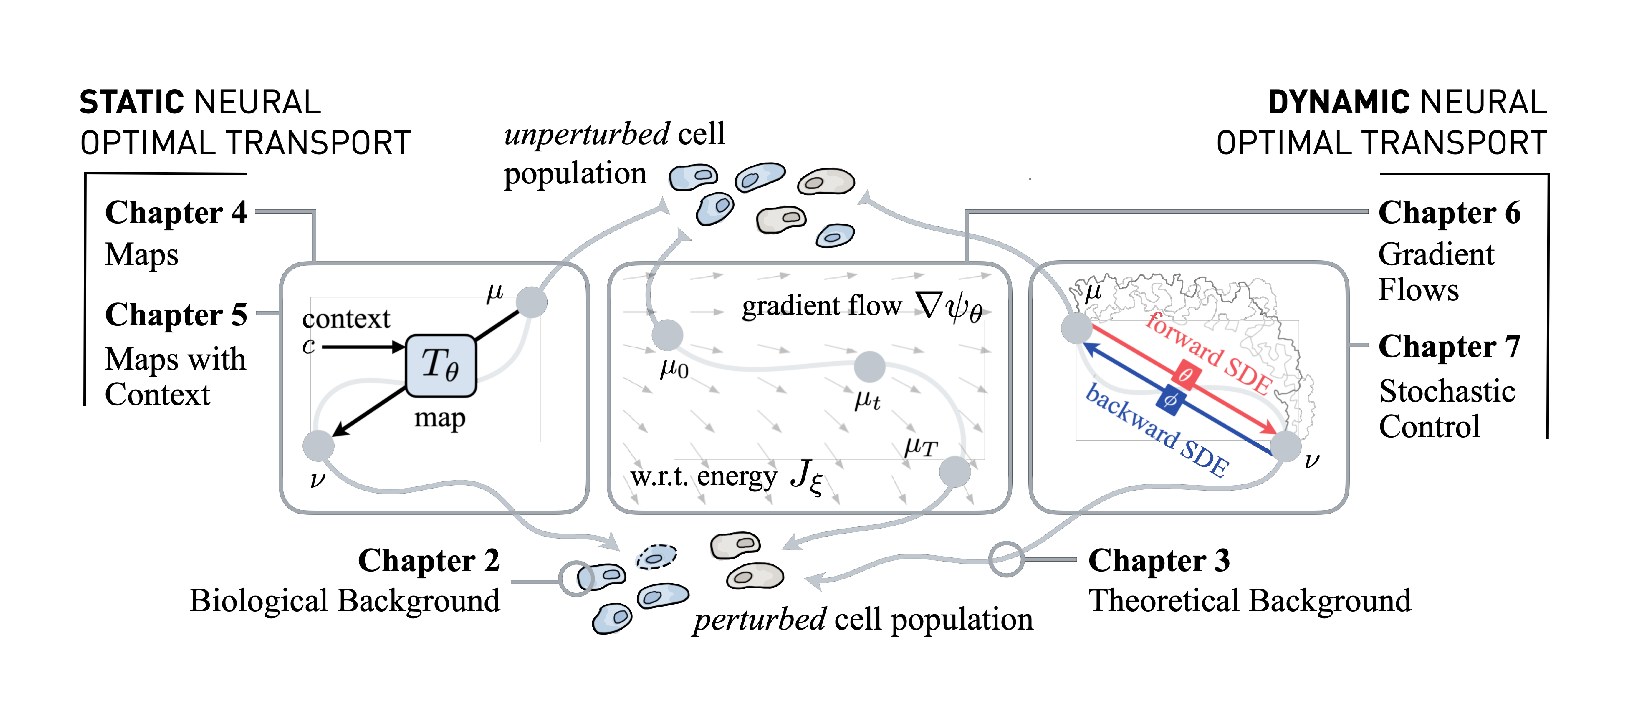
\includegraphics[width=\textwidth]{figures/fig_overview_thesis.pdf}
  \caption{Structure of the thesis with references to the chapters.}
  \label{fig:overview_thesis}
\end{figure}

\section{Scope and Contributions}

In this thesis, we introduce and design novel deep learning architectures capable of modeling heterogeneous population dynamics from unaligned snapshot data.
A framework that facilitates the design of such deep learning architectures that (\colcircle{pink}) operate on distributions, i.e., allows modeling heterogeneous populations of particles, (\colcircle{lightblue}) trained based on samples of \emph{unaligned} distributions is the \textbf{theory of optimal transport}.

The mathematical foundation of this work further builds on the intuition that perturbations incrementally alter the molecular profiles of cells. This underlying assumption aligns with the theory of \acrfull{OT} that studies the evolution of measures under the \emph{minimum effort} principle. Thus, (\colcircle{darkblue}) OT serves naturally as an inductive bias of the deep learning architectures introduced in this thesis.
By providing tools for modeling the evolution of distributions over time, OT allows us to reconstruct and predict the incremental changes in cell states upon perturbation such as therapeutic agents or developmental signals. 
In recent years, OT has enabled significant advances in single-cell biology problems \citep{schiebinger2019optimal, lavenant2021towards, demetci2022scot}. However, traditional OT methods do not enable predictions for unperturbed cells that have not been previously observed.
They are thus unable to predict perturbation responses out-of-sample, e.g., of cells from new incoming samples, such as those from unseen patients. 
This thesis is thus concerned with the development of so-called  (\colcircle{blue}) \textbf{neural optimal transport} that allow for out-of-sample \emph{predictions} on unseen cells and \emph{forecasting} of cellular dynamics \citep{makkuva2020optimal, tong2020trajectorynet,  korotin2021wasserstein, bunne2022proximal, bunne2022supervised, bunne2021learning}. \\

Optimal transport comes in many different flavors and has strong mathematical roots in dynamic systems theory.
The goal of the \emph{static} formulation of OT is thereby to identify a map that \emph{optimally} morphs or transports a distribution onto another, and thus "best" explains the one-step evolution of a measure.
The static framework, however, has an immediate dynamic formulation. By introducing a time-variable into this \emph{transport}, OT allows us to study the continuous evolution of a measure over time. % , critical when aiming at interpolating between different measurements.
Importantly, generalizations of this \emph{dynamic} formulations can be formalized through ordinary, partial, or stochastic differential equations. Building on recent innovations in neural \acrfullpl{ODE} \citep{chen2018neural} and more recently flow matching models \citep{lipman2023flow, pooladian2023multisample, liu2022flow}, as well as \acrfullpl{SDE}-based neural networks 
This thesis will explore the full palette of ...

The thesis is structured as follows (see outline in \cref{fig:overview_thesis}).
After reviewing dynamical systems in biomedicine in \cref{cha:bio_background} and providing a mathematical foundation of static and dynamic optimal transport in \cref{cha:theory_background}, the \textbf{thesis contributions} are then organized in two parts:

\paragraph{\cref{part:static_not}: Static neural optimal transport.}

At its core it defines a so-called \citeauthor{monge1781histoire} \textit{map}, which provides an actionable way to flow from one probability distribution onto another.
The design of neural network-parameterizations of such maps and their application to predict perturbation responses of single-cells will form the first contribution of this thesis.
This comprises approaches that are a direct consequence of the famous \citeauthor{brenier1987decomposition} theorem, and allow us to model Monge maps as gradients of convex functions \citep{bunne2021learning, bunne2022supervised}.

More concretely, \cref{part:static_not} comprises two chapters:
\cref{cha:cellot} ... \citep{bunne2021learning}. To ..., \cref{cha:condot} ... \citep{bunne2022supervised}.
... \\
	
\textbf{Applications:} Predicting responses of heterogeneous cell populations to molecular perturbations (e.g., genetic knockouts or overexpression, chemical drugs, or developmental signals) at the level of single cells
% A fundamental difficulty is thus to reconstruct perturbation responses of individual cells from a set of unaligned unperturbed and perturbed cells. To forecast patient cell reactions to treatments or deduce cell differentiation paths, we need to reconcile these unpaired snapshots, thus predicting each cell's perturbed state.


\paragraph{\cref{part:dynamic_not}: Dynamic neural optimal transport.}
This part subsequently covers methods within the dynamic neural optimal transport framework. 

Beyond mappings, OT provides a mathematical link to geometric variational frameworks that allow studying flows of distributions on metric spaces.
In particular, \citeauthor{brenier1987decomposition}'s dynamical formulation of OT has given rise to a flurry of applications studying \acrfullpl{PDE} as gradient flows or steepest descent in spaces of probability measures.
\citet*{benamou2000computational} showed how the dynamic point of view offers an alternate and intuitive interpretation of optimal transport with links to fluid dynamics that surprisingly leads to a convex optimization problem that can be parameterized through normalizing flows \citep{tong2020trajectorynet}.
We will further highlight connections of OT to PDEs such as Fokker-Planck-like equations through the \citeauthor*{jordan1998variational} scheme: In recent works \citep{bunne2022proximal, alvarez2021optimizing, mokrov2021large, benamou2016augmented} 
it has found application in inferring the evolution of populations over time, crucial in many scientific disciplines when for instance, observing a population of cells in biology.

In particular, \cref{cha:neural_pde} ... \citep{bunne2022proximal}.

Lastly, beyond PDEs, this thesis explores the relation between the optimal transport problem and the \acrfull{SB} problem from stochastic control. It represents a key connection that has recently fueled the development of \acrfull{DSB} \citep{de2021diffusion, chen2021stochastic, liu2022deep, bunne2022recovering}. \\

\cref{cha:neural_sde} ...
\cref{sec:gsbflow} ... \citep{bunne2022recovering}.
\cref{sec:sbalign} ... \citep{somnath2023aligned}.
... \\

\textbf{Applications:} ...


\section{Publications}
All results presented in this thesis have been published in the following conference proceedings and journals:

\begin{itemize}
	\item[] Charlotte Bunne, Laetitia Meng-Papaxanthos, Andreas Krause, and Marco Cuturi. Proximal Optimal Transport Modeling of Population Dynamics. In \textit{International Conference on Artificial Intelligence and Statistics (AISTATS)}, volume 25, 2022.
	\item[] Charlotte Bunne, Andreas Krause, and Marco Cuturi. Supervised Training of Conditional Monge Maps. In \textit{Advances in Neural Information Processing Systems (NeurIPS)}, 2022.
	\item[] Charlotte Bunne, Ya-Ping Hsieh, Marco Cuturi, and Andreas Krause. The Schr{\"o}dinger Bridge between Gaussian Measures has a Closed Form. In \textit{International Conference on Artificial Intelligence and Statistics (AISTATS)}, 2023.
	\item[] Vignesh Ram Somnath, Matteo Pariset, Ya-Ping Hsieh, Maria Rodriguez Martinez, Andreas Krause, and Charlotte Bunne. Aligned Diffusion Schr{\"o}dinger Bridges. In \textit{Conference on Uncertainty in Artificial Intelligence (UAI)}, 2023.
	\item[] Charlotte Bunne, Stefan G Stark, Gabriele Gut, Jacobo Sarabia del Castillo, Kjong-Van Lehmann, Lucas Pelkmans, Andreas Krause, and Gunnar R{\"a}tsch. Learning Single-Cell Perturbation Responses using Neural Optimal Transport. \textit{Nature Methods}, 2023.
\end{itemize}

\paragraph{Further publications.}
The following publications of the author and collaborators are more broadly relevant to the topic of this thesis but have not been directly included:

\begin{itemize}
	\item[] Charlotte Bunne, David Alvarez-Melis, Andreas Krause, and Stefanie Jegelka. Learning Generative Models across Incomparable Spaces. In \textit{International Conference on Machine Learning (ICML)}, 2019.
	\item[] Matteo Manica, Charlotte Bunne, Roland Mathis, Joris Cadow, Mehmet Eren Ahsen, Gustavo A Stolovitzky, and Maria Rodriguez Martinez. COSIFER: a Python package for the consensus inference of molecular interaction networks. \textit{Bioinformatics}, 37(14), 2020.
	\item[] Vignesh Ram Somnath, Charlotte Bunne, Connor Coley, Andreas Krause, and Regina Barzilay. Learning Graph Models for Retrosynthesis Prediction. In Advances in Neural Information Processing Systems (NeurIPS), 2021.
	\item[] Vignesh Ram Somnath, Charlotte Bunne, and Andreas Krause. Multi-Scale Representation Learning on Proteins. In \textit{Advances in Neural Information Processing Systems (NeurIPS)}, 2021.
	\item[] Marco Cuturi, Laetitia Meng-Papaxanthos, Yingtao Tian, Charlotte Bunne, Geoff Davis, and Olivier Teboul. Optimal Transport Tools (OTT): A JAX Toolbox for all things Wasserstein. \textit{arXiv Preprint arXiv: 2201.12324}, 2022.
	\item[] Octavian-Eugen Ganea, Xinyuan Huang, Charlotte Bunne, Yatao Bian, Regina Barzilay, Tommi S. Jaakkola, and Andreas Krause. Indepen- dent SE(3)-Equivariant Models for End-to-End Rigid Protein Docking. In \textit{International Conference on Learning Representations (ICLR)}, 2022.
	\item[] Philippe Schwaller, Alain C Vaucher, Ruben Laplaza, Charlotte Bunne, Andreas Krause, Clemence Corminboeuf, and Teodoro Laino. Machine intelligence for chemical reaction space. \textit{Wiley Interdisciplinary Reviews: Computational Molecular Science}, 2022.
	\item[] Frederike L\"ubeck, Charlotte Bunne, Gabriele Gut, Jacobo Sarabia del Castillo, Lucas Pelkmans, and David Alvarez-Melis. Neural Unbalanced Optimal Transport via Cycle-Consistent Semi-Couplings. \textit{arXiv Preprint arXiv: 2209.15621}, 2022.
	\item[] Matteo Pariset, Ya-Ping Hsieh, Charlotte Bunne, Andreas Krause, and Valentin De Bortoli. Unbalanced Diffusion Schr{\"o}dinger Bridge. \textit{arXiv Preprint arXiv: 2306.09099}, 2023.
\end{itemize}

\section{Collaborators}

This thesis would not have been possible without my advisors, Andreas Krause and Marco Cuturi, and many of the ideas presented here have been shaped in our meetings. I further enjoyed collaborating with my colleagues on numerous ideas, and the results presented and not otherwise cited are by the author and collaborators. In particular, \cref{cha:cellot} contains material of a publication with shared first authorship between the author, Stefan Stark, and Gabriele Gut. Besides Andreas Krause, the corresponding authors are Kjong-Van Lehmann, Lucas Pelkmans, and Gunnar R\"atsch.
\cref{sec:gsbflow} is based on a joint first authorship project with Ya-Ping Hsieh who contributed the theoretical analysis of that work. Lastly, \cref{sec:sbalign} contains material from a publication where Vignesh Ram Somnath and Matteo Pariset share the first authorship while the author serves as corresponding author.



\chapter{Dynamic Processes in Biomedicine}
\label{cha:bio_background}

\dictum[Rosalind Franklin, \textit{Report} (1952)]{%
  The results suggest a helical structure (which must be very closely packed) containing probably 2, 3, or 4 coaxial nucleic acid chains per helical unit and having the phosphate groups near the outside.}%
\vskip 2em

Dynamical processes, with their inherently complex and constantly changing patterns of interactions and behaviors, are fundamental to every function of life, from the oscillatory rhythms of cellular processes to the broader orchestration of biological systems.
This involves an array of intricate interactions between molecules, genes, cells, tissues, and their biophysical environment. They span a multitude of scales and dimensions --- spatial as well as temporal.
Early events in cell signaling, for example, often start within seconds after the stimulus, followed by intracellular signaling and transcription changes over minutes to hours. In contrast, cell fate decisions like division, differentiation, or apoptosis can take many hours or days to manifest \citep{spiller2010measurement}.
Measuring and modeling these inherently stochastic dynamics is critical to the effective understanding of biological systems and the subsequent development of diagnostic and therapeutic tools.
However, they are equally daunting, demanding novel experimental and computational strategies.

This section of the thesis will delve into the exploration of two examples of dynamic processes in biomedicine that are subject of this thesis. 
In particular, we will focus on the analysis of cellular responses to perturbations such as drugs or other therapeutic agents (\cref{sec:cell_perturbation_responses}) as well as cell differentiation processes in developmental biology (\cref{sec:cell_differentiation}), and illuminate the critical role they play in biomedicine and the myriad of challenges and opportunities they present. 
This will be followed by a discussion on current advances in high-throughput technologies for capturing such dynamical systems (\cref{sec:tech_background}) and existing computational approaches to tackle these (\cref{sec:related_work_bio}).

\section{Cellular Perturbation Responses to Drugs and Treatments}
\label{sec:cell_perturbation_responses}

% TODO: Add more citations.
A fundamental task in personalized medicine involves predicting outcomes and responses of patients to potential treatments in order to subsequently select the most effective therapy based on the patient biopsies or tissue culture during screens.
A key aspect of biomedical research thus concerns the study of cellular perturbation responses to therapeutic agents, including drugs and other treatments. 
Perturbations such as small molecule drugs can thereby have profound effects on the biological \emph{phenotype} that responds in complex and often unpredictable ways.
Such responses might range from the induction of apoptosis to changes in cellular proliferation, migration, differentiation, and metabolism, each significantly affecting the overall state of the organism. 
Perturbations can also trigger cascade effects across interrelated signaling pathways, leading to a state of cellular disequilibrium.

As populations of cells are almost always \emph{heterogeneous} in function and fate and subsequently, their response to a perturbation strongly vary, where different cell states exhibit distinct sensitivities toward a external stimuli \citep{spiller2010measurement}.
Heterogeneity is particular inherent in cancer and fuel for resistance: Genomic instability, which can range in magnitude from single-base substitutions to whole-genome doublings, is critical to the development and progression of many cancers \citep{dagogo2018tumour}. Understanding diverging behavior of tumor cells toward a therapy is crucial in order to understand the underlying mechanisms of cellular sensitivities and \emph{resistance}.

Thus, understanding responses of individual cells and distinct cell states to perturbations is crucial as they can illuminate mechanisms of drug efficacy and potential side effects.
At the same time it reveals potential targets for improved therapeutic strategies. 

Most of these effects depend on the context in which the perturbation occurs. Given the heterogeneity among single cells in cell populations and tissues, predicting cellular responses requires understanding the rules by which context shapes genome activity and its response to drugs. High-dimensional single-cell data measured via single-cell genomics or multiplexed imaging technologies can provide this contextual information but only return unpaired or unaligned observations of cell populations.
In order to understand how an unperturbed population $\mu$ responds and evolves into the perturbed population $\nu$, we need to recover a map $T$ that describes the perturbation effect. Parameterizing this through a neural network allows us to predict how a cell $x$ changes upon perturbation $y= T(x)$ (see \cref{fig:bio_problems}a).

% However, capturing this cellular responsiveness presents considerable challenges due to the heterogeneity of individual cells, the dynamism of biological systems, and the multi-dimensional interactions occurring within and across cells.

% Recent high-throughput methods provide great insights on how cell populations respond to various perturbations on the level of individual cells. The provided data, however, is non-time-resolved and unaligned. 
% Hence, snapshots taken of biological samples before and after perturbations do not provide information on single-cell trajectories.
% Perturbations might include the application of drugs affecting molecular functions in cells, or changes in the cellular environment causing shifts in biological signaling, thus impacting cells and their states in various ways.

\begin{figure}[t]
  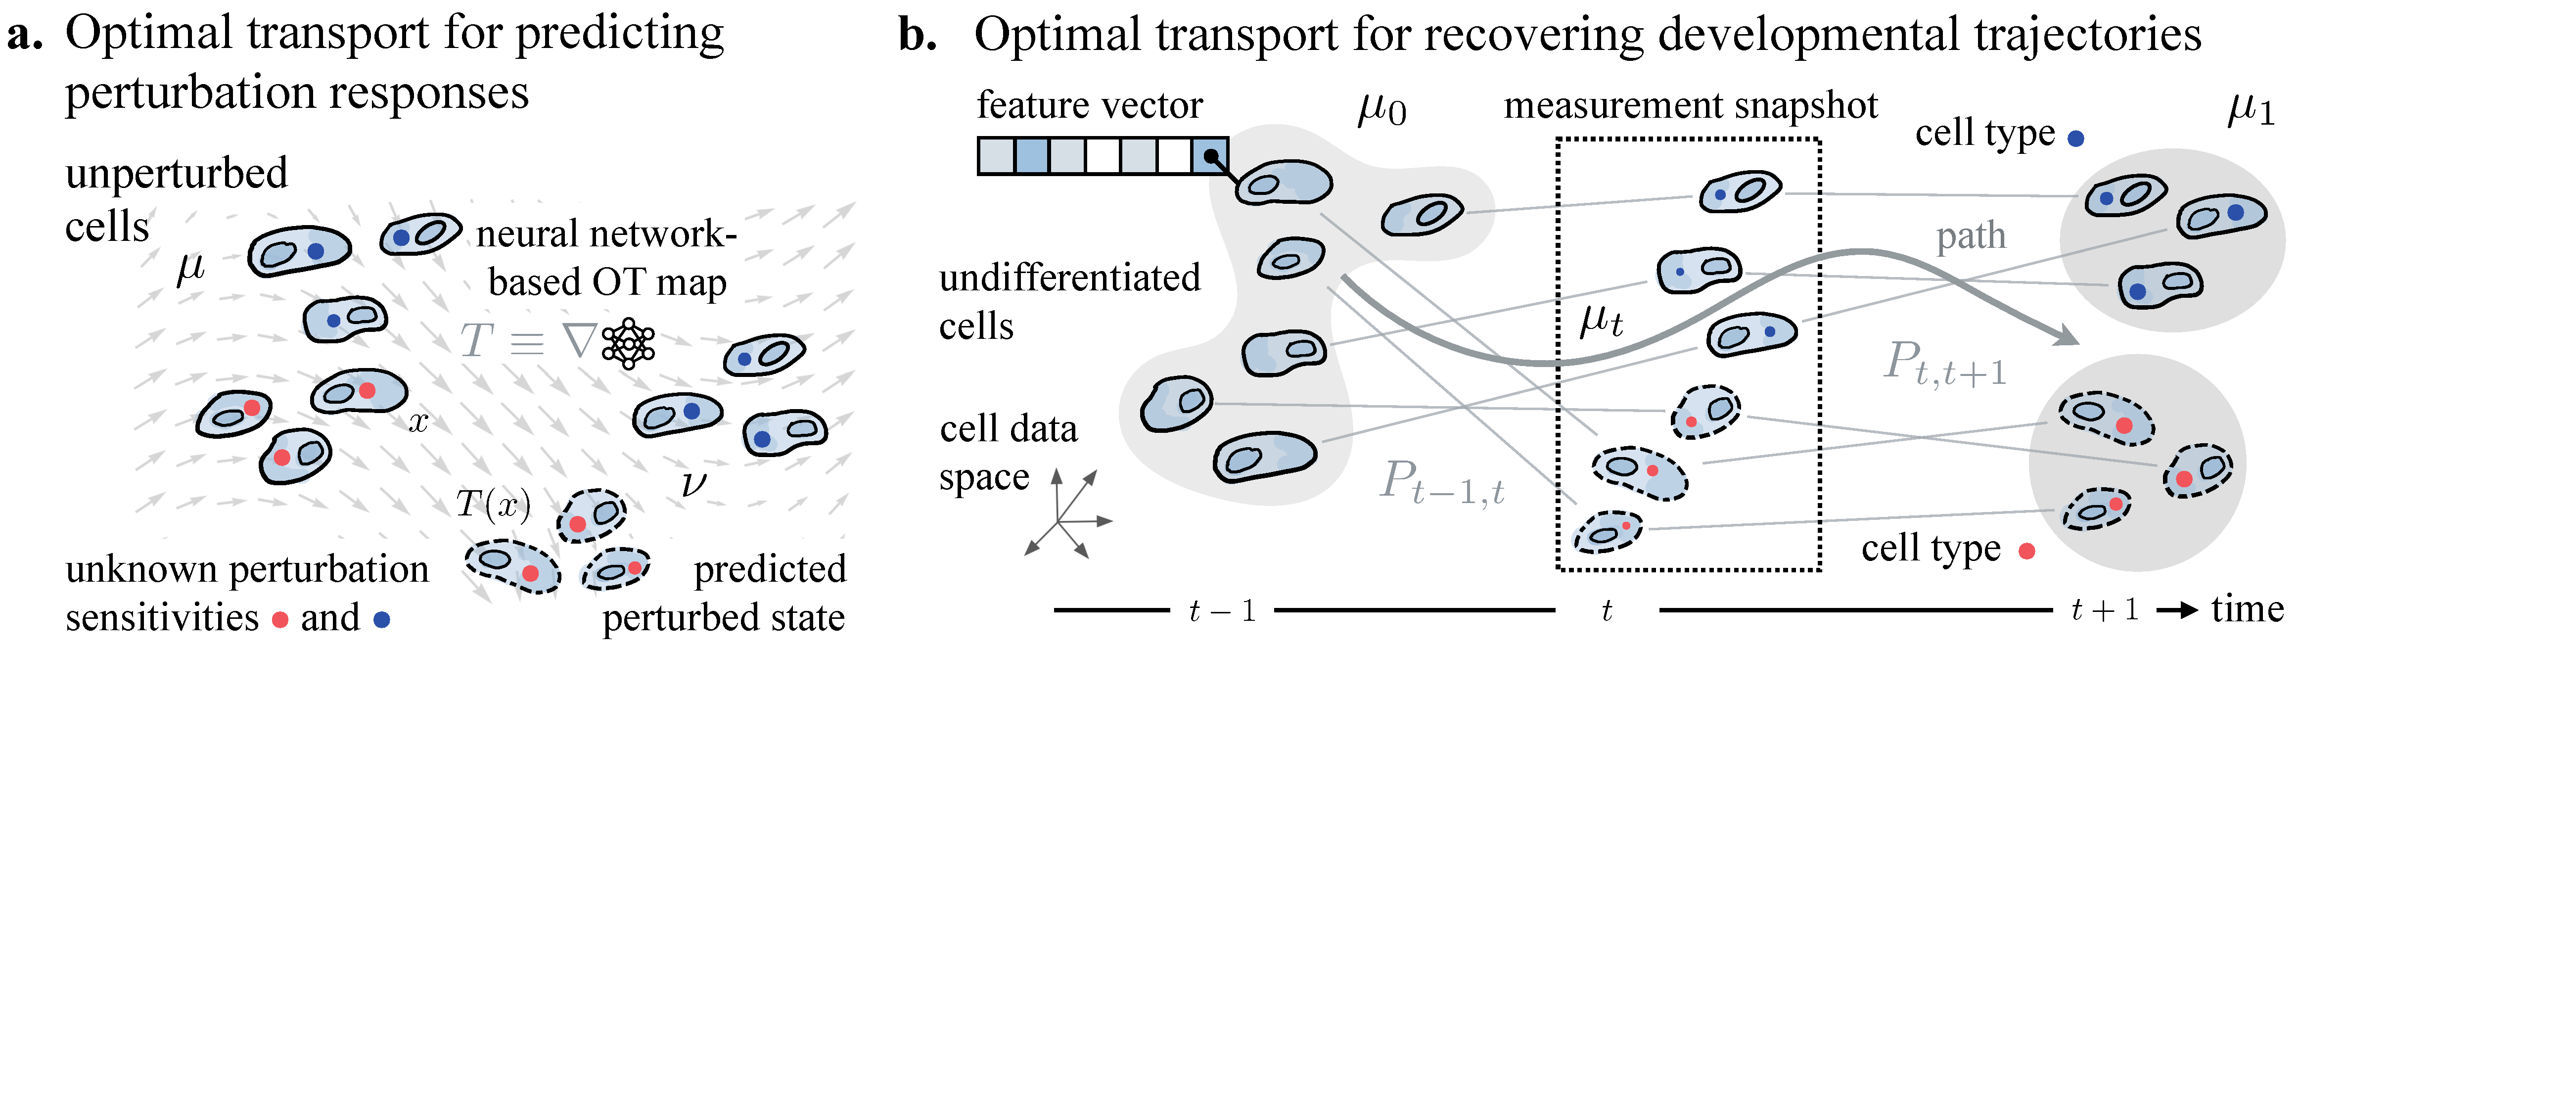
\includegraphics[width=\textwidth]{figures/fig_bio_problems.pdf}
  \caption{\textbf{Overview on different dynamical processes in biomedicine.} \textbf{a.} In order to understand and predict the response of an unperturbed cell population $\mu$ to a stimulus such as a therapeutic agent, we need to identify a map $T$ that explains its evolution into the perturbed population $\nu$. Then, the perturbed state of a cell $x$ is given by $T(x)$.  \textbf{b.} Developmental processes describe the evolution of a often homogeneous population of undifferentiated cells into various cell lineages. Reconstructing such processes from measurement snapshots can be achieved through sequential alignments $P_{t-1,t}$ that describe the evolution from $\mu_0$ to $\mu_1$, or by identifying the overall global path $\mu_t$ capturing the cell differentiation process.}
  \label{fig:bio_problems}
\end{figure}

\section{Cell Differentiation and Lineage Tracing in Developmental Biology}
\label{sec:cell_differentiation}

Complex cellular dynamics are not only initiated through external stimuli, but also at the core of developmental processes, tissue regeneration and formation.
The spectacular journey of a single zygote in the embryonic development, for example, metamorphosing into a complex, multicellular organism is largely governed by the mechanisms of cell differentiation, where pluripotent stem cells commit to specific lineages and mature into diverse cell types.

Understanding the molecular programs that guide such differentiation processes is a major challenge.
% Lineage tracing serves as a powerful tool to retrospectively track the genealogical origin of cells, helping to construct an in-depth chronicle of cellular development and differentiation. It unravels the developmental trajectory of cells, thereby facilitating the understanding of normal development as well as pathological conditions.
% However, capturing this process with accuracy poses profound challenges due to the stochastic nature of cell differentiation, technical complexities, and the vast temporal and spatial scales involved.
However, approaches relying on the bulk analysis of cell populations fall short in tackling these issues, as they fail to offer comprehensive solutions to two key obstacles: identifying various cell types within a population and tracking the development of each of these types.
By providing insights into the heterogeneity of cell populations, single-cell methods partially address the aforementioned challenges, but their destructive nature impedes the recording of the expression of the same cell and its direct descendants across time.
Hence, such differentiation processes can only be measured through distinct snapshots of single-cell populations that are \textit{not time-resolved} and \textit{unaligned}.

To understand differentiation ---the continuous emergence of different cell types and branching events--- we need to reconstruct such developmental processes from single-cell measurements that provide us with snapshots of the cell population evolving over time:
Given that a cell has a specific expression profile at a time point, where will its descendants likely be at a later time point and where are its likely ancestors at an earlier time point? 
\citet{schiebinger2019optimal} for example study reprogramming of fibroblasts to \acrfull{iPSC} \citep{takahashi2006induction}, by measuring \acrfull{MEF}. Cells at time point $t$ are connected to their ancestors at time $t-1$, by finding the corresponding transport plan $P_{t-1,t}$ between each pair of consecutive time steps (see \cref{fig:bio_problems}b).
To understand the overall dynamic process, however, this thesis aims at identifying the overall dynamic evolution of measure $\mu_t$ instead of resorting to the computation of distinct alignments between consecutive measurement snapshots \citep{lavenant2021towards}.


\section{Single-Cell High-Throughput Technologies}
\label{sec:tech_background}

Until recently, our understanding of cellular dynamics was limited to 'bulk' omics analyses, which yield average measurements for a cell population.
The advent of single-cell omics technologies has marked a significant shift from such average analyses, enabling a highly detailed examination of individual cells across various layers such as the genome, transcriptome, epigenome, and proteome.
This shift has revealed previously hidden complexities, such as rare cell types, transitional states, and cell-to-cell variability. Transformative techniques like single-cell RNA sequencing (\cref{sec:background_sequencing}) have allowed researchers to profile gene expression in thousands of cells simultaneously, shedding light on new cellular subpopulations and responses \citep{jia2022high}.
Additionally, modern imaging technologies have deepened our understanding of cell morphology and (the localization of) cellular signaling (\cref{sec:background_imaging}). 
The integration of these diverse omics layers provides a holistic view of cellular diversity, opening new avenues in the study of health, disease, and personalized medicine \citep{baysoy2023technological}.

Each point $x$ of such single-cell measurements then represents the recorded features of a single cell. Each feature (dimension) of that point tracks the expression level of each studied gene, or morphological and signaling feature strength in that cell, at measurement time. In this setting, a few thousand cells are sampled from a large population of cells, to obtain their features (high-throughput). This is done at distinct time points throughout cellular processes. Because of the destructive process of these measurements, each snapshot consists of several feature vectors, one for each different cell.
Two consecutive snapshots can be seen as two point clouds % that capture the heterogeneity of cells at each point in time. 
or, alternatively, as two tabular datasets $X = [x_1,\dots, x_n]$ and $Y=[y_1, \dots, y_m]$: Each of the $n$ or $m$ rows contains a cell and its $d$-dimensional feature representation, where each column denotes a particular feature, e.g., the activity of a gene.
In order to understand the temporal evolution of the cell population over time, we aim to provide an informed guess on an alignment or a map that relates the two cell populations $X$ and $Y$.
% In the following, we will discuss two different high-throughput technologies that allow us to record such features.

\subsection{Sequencing-Based Screening}
\label{sec:background_sequencing}

Sequence-based profiling methods have emerged as a transformative tool for understanding the complexity of biological systems at the resolution of individual cells. Methods such as single-cell \acrlong{RNA-seq} (scRNA-seq) or single-cell \acrlong{ATAC-seq} (scATAC-seq), enable us to characterize gene expression or chromatin accessibility within a single cell.
By mapping the transcriptomic or epigenomic landscapes of individual cells, sequence-based profiling methods have allowed for unprecedented insights into developmental biology, tissue homeostasis, disease pathology, and therapeutic responses.

RNA thereby serves a direct quantifier for gene activity: Genes in DNA are transcribed into \acrfull{mRNA}, which is then translated into proteins that carry out various functions within the cell.
By measuring the amounts and types of mRNA present in a cell at a given time, i.e., the transcriptome, we can understand which genes are being actively expressed. This information is valuable as changes in gene expression can signal various biological processes, such as cell development, responses to environmental stimuli, disease states, and much more. 
In order to record the gene expression in single cells, scRNA-seq requires isolating individual cells, often using techniques such as \acrfull{FACS} \citep{julius1972demonstration} or droplet-based technologies \citep{brouzes2009droplet, mazutis2013single, debs2012functional}. Each cell's mRNA is reverse transcribed into \acrfull{cDNA}, including a unique molecular identifier to correct for amplification bias.
This cDNA is then amplified and prepared for high-throughput sequencing and the resultant data provide insights into gene expression of individual cells.

Crucially, this process is destructive: Cells are destroyed, i.e., lysed, or broken open, in order to access the mRNA within and record their gene expression levels.
Once a cell is lysed, its structural integrity and function are lost, making it impossible to further manipulate or use that particular cell for subsequent experiments.
This is a fundamental limitation, as the process of obtaining the high-resolution molecular data comes at the expense of the cell's viability.

\subsection{Optical Phenotypic Screening}
\label{sec:background_imaging}

Optical phenotypic screening allows for the analysis of single cells based on their morphological and biochemical characteristics, with minimal perturbation to their natural state. 
Techniques such as fluorescence microscopy, time-lapse imaging, or flow cytometry typically involve labeling cells with fluorescent dyes or proteins that bind to or are expressed by specific cellular components of interest.
Such targets tagged with markers can be potential important components of signaling pathways or crucial regulators and indicators of core cellular functions. 
The cells are then imaged or passed through a laser, and the fluorescence emitted is captured and measured, providing information about the presence and quantity of the target molecules within each cell. 
The resulting images allow the extraction of morphological properties and the fluorescence intensity of each tag in different parts of each cell \citep{carpenter2006cellprofiler}.

However, it's important to note that while these methods are in general non-destructive in nature, some processes such as labeling or the use of certain dyes could potentially have some impact on cell viability or behavior. So while these techniques in general allow for dynamic tracking of cellular processes \citep{fischer2019inferring, hashimoto2016learning, tvarusko1999time, busch2015fundamental}, cells are usually fixed prior to staining to preserve cellular structures and allow for longer-term storage. Such procedures are lethal for cells, making longitudinal studies on the same cells impossible.

High-content imaging, particularly when augmented by multiplexing abilities, is ideally suited to study heterogeneous cell responses.
In this thesis, we study heterogeneous cell line responses to various cancer drugs based on a measurement technology known as \acrfull{4i} \citep{gut2018multiplexed}.
With 4i, fluorescently labeled antibodies are iteratively hybridized, imaged, and removed from a sample to measure the abundance and localization of proteins and their modifications. 
Thus, 4i quickly generates large, spatially resolved phenotypic datasets rich in molecular information from thousands of treated and untreated cells. Additionally to the multiplexed information generated by 4i, cellular and nuclear morphology are routinely extracted from microscopy images (without the need for 4i) by image analysis algorithms \citep{carpenter2006cellprofiler}.

% \section{Related Work on Studying Cell Dynamics}

% ...
% \citep{fischer2019inferring, busch2015fundamental, hashimoto2016learning, raue2015data2dynamics}

\section{Optimal Transport for Single-Cell Biology}
% TODO: Change labels if above section is written.
\label{sec:related_work_bio}
\label{sec:ot_for_biology}

Applied to the analysis and modeling of single-cell biology problems, OT has been used to infer the distributions of cells' ancestors and descendants along development \citep{schiebinger2019optimal}, perform trajectory inference \citep{bunne2022proximal, forrow2021lineageot, bunne2022recovering, lavenant2021towards, schiebinger2019optimal, tong2020trajectorynet, yang2020predicting, zhang2021optimal, chizat2022trajectory}, predict perturbation responses \citep{bunne2021learning, yang2018scalable, lubeck2022neural}, integrate multi-omics data of different modalities \citep{demetci2022scot}, infer cell-cell similarity \citep{huizing2022optimal}, and integrate across scales (e.g., morphology and molecular profiling) \citep{yang2021multi}. The increasing data complexity across multiple levels of biological organization, from molecular and cellular through spatial profiling \citep{moriel2021novosparc} of tissues, and imaging of organs, cement further the status of OT as an indispensable framework for high-throughput, multimodal, and multi-scale molecular, cell, tissue, and organ biology. The effectiveness of OT comes, however, with drawbacks: because the theory builds on extremely sophisticated mathematics that blends optimization \citep{cuturi2013sinkhorn, cuturi2022optimal}, stochasticity \citep{chizat2022trajectory, bunne2022recovering} and partial differential equations \citep{bunne2022proximal}, and, more recently, deep learning \citep{tong2020trajectorynet, bunne2021learning, bunne2022supervised, yang2018scalable, lubeck2022neural, yang2021multi}, its computations are challenging even by modern ML standards.
